% ---------------------------------------------------------------------
% -------------- PREAMBLE ---------------------------------------------
% ---------------------------------------------------------------------
\documentclass[12pt,a4paper,finnish,oneside]{article}
%\documentclass[12pt,a4paper,finnish,twoside]{article}
%\documentclass[12pt,a4paper,finnish,oneside,draft]{article} % luonnos, nopeampi

% Valitse 'input encoding':
%\usepackage[latin1]{inputenc} % merkistökoodaus, jos ISO-LATIN-1:tä.
\usepackage[utf8]{inputenc}   % merkistökoodaus, jos käytetään UTF8:a
% Valitse 'output/font encoding':
%\usepackage[T1]{fontenc}      % korjaa ääkkösten tavutusta, bittikarttana
\usepackage{ae,aecompl}       % ed. lis. vektorigrafiikkana bittikartan sijasta
% Kieli- ja tavutuspaketit:
\usepackage[english,swedish,finnish]{babel}
% Kurssin omat asetukset aaltosci_t.sty:
\usepackage{aaltosci_t}
% Jos kirjoitat muulla kuin suomen kielellä valitse:
%\usepackage[finnish]{aaltosci_t}           
%\usepackage[swedish]{aaltosci_t}           
%\usepackage[english]{aaltosci_t}           
% Muita paketteja:
\usepackage{alltt}
\usepackage{amsmath}   % matematiikkaa
\usepackage{calc}      % käytetään laskurien (counter) yhteydessä (tiedot.tex)
\usepackage{eurosym}   % eurosymboli: \euro{}
\usepackage{url}       % \url{...}
\usepackage{listings}  % koodilistausten lisääminen
\usepackage{algorithm} % algoritmien lisääminen kelluvina
\usepackage{algorithmic} % algoritmilistaus
\usepackage{hyphenat}  % tavutuksen viilaamiseen liittyvä (hyphenpenalty,...)
\usepackage{supertabular,array}  % useampisivuinen taulukko
\usepackage{hyperref}
% Koko dokumentin kattavia asetuksia:

% Tavutettavia sanoja:
%\hyphenation{vää-rin me-ne-vi-en eri-kois-ten sa-no-jen tavu-raja-ehdo-tuk-set}
% Huomaa, että ylläoleva etsii tarkalleen kyseisiä merkkijonoja, eikä
% ymmärrä taivutuksia. Paikallisesti tekstin seassa voi myös ta\-vut\-taa.

% Rangaistaan tavutusta (ei toimi?! Onko hyphenat-paketti asennettu?)
\hyphenpenalty=10000   % rangaistaan tavutuksesta, 10000=ääretön
\tolerance=1000        % siedetään välejä riveillä
% titlesec-paketti auttaa, jos tämän mukana menee sekaisin

% Tekstiviitteiden ulkoasu.
% Pakettiin natbib.sty/aaltosci.bst liittyen katso esim. 
% http://merkel.zoneo.net/Latex/natbib.php
% jossa selitykset citep, citet, bibpunct, jne.
% Valitse alla olevista tai muokkaa:
\bibpunct{(}{)}{;}{a}{,}{,}    % a = tekijä-vuosi (author-year)
%\bibpunct{[}{]}{;}{n}{,}{,}    % n = numero [1],[2] (numerical style)

% Rivivälin muuttaminen:
\linespread{1.24}\selectfont               % riviväli 1.5
%\linespread{1.24}\selectfont               % riviväli 1, kun kommentoit pois

% ---------------------------------------------------------------------
% -------------- DOCUMENT ---------------------------------------------
% ---------------------------------------------------------------------

\begin{document}

% -------------- Tähän dokumenttiin liittyviä valintoja  --------------

%\raggedright         % Tasattu vain vasemmalta, ei tavutusta
% ----------------- joitakin makroja ----------------------------------
%
% \newcommand{\sinunKomentosi}[argumenttienMäärä]{komennot%
% voiJakaaRiveille%
% jaArgumenttienViittaus#1,#2,#argumenttienMäärä}

% Joskus voi olla tarpeen kommentoida jotakin. Ei suositella. 
% Äläkä unohda lopulliseen! 
\newcommand{\Kommentti}[1]{\fbox{\textbf{OMA KOMMENTTI:} #1}}
% Käyttö: Kilometri on 1024 metriä. \Kommentti{varmista tämä vielä}.
% Eli newcommand:n komentosanan jälkeen hakasaluissa argumenttien lkm,
%  ja argumentteihin viitataa #1, #2, ...

%  Comment out this \DRAFT macro if this version no longer is one!  XXX
%\newcommand{\DRAFT}{\begin{center} {\it DRAFT! \hfill --- \hfill DRAFT!
%\hfill --- \hfill DRAFT! \hfill --- \hfill DRAFT!}\end{center}}

%  Use this \DRAFT macro in the final version - or comment out the 
%  draft-command
% \newcommand{\DRAFT}{~}

% %%%%%%%% MATEMATIIKKA %%%%%%%%%%%%%%%%%

% Määrätty integraali
\newcommand{\myInt}[4]{%
\int_{#1}^{#2} #3 \, \textrm{d}{#4}}

% http://kapsi.fi/jks/satfaq/
%\newcommand{\vii}{\mathop{\Big/}}
%\newcommand{\viiva}[2]{\vii\limits_{\!\!\!\!{#1}}^{\>\,{#2}}}
%%\[ \intop_0^{10} \frac{x}{x^2+1} \,\mathrm{d}x
%%= \viiva{0}{10} \frac{1}{2}\ln(x^2+1) \]

% matht.sty, Simo K. Kivelä, 01.01.2002, 07.04.2004, 19.11.2004, 21.02.2005
% Kokoelma matemaattisten lausekkeiden kirjoittamista helpottavia
% määrittelyjä.

% 07.04.2004 Muutama lisäys ja muutos tehty: \ii, \ee, \dd, \der,
% \norm, \abs, \tr.
%
% 19.11.2004 Korjattu määrittelyjä: \re, \im, \norm;
% lisätty \trp (transponointi), \hrm (hermitointi), \itgr (rakenteellinen
% integraali), ympäristö Cmatrix (hakasulkumatriisi);
% vanha transponointi \tr on mukana edelleen, mutta ei suositella.

% Pakotettu rivinvaihto, joka voidaan tarvittaessa määritellä
% uudelleen: 

%\newcommand{\nl}{\newline}

% Logiikan symboleja (<=> ja =>) hieman muunnettuina:

%\newcommand{\ifftmp}{\;\Leftrightarrow\;}
%\newcommand{\impltmp}{\DOTSB\;\Rightarrow\;}

% 'siten, että' -lyhenne ja hattupääyhtäläisyysmerkki vastaavuuden
% osoittamiseen: 

%\newcommand{\se}{\quad \text{siten, että} \quad}
%\newcommand{\vs}{\ {\widehat =}\ }

% Lukujoukkosymbolit:

%\newcommand{\N}{\ensuremath{\mathbb N}}
%\newcommand{\Z}{\ensuremath{\mathbb Z}}
%\newcommand{\Q}{\ensuremath{\mathbb Q}}
%\newcommand{\R}{\ensuremath{\mathbb R}}
%\newcommand{\C}{\ensuremath{\mathbb C}}

% Reaali- ja imaginaariosa, imaginaariyksikkö:

%\newcommand{\re}{\operatorname{Re}}
%\newcommand{\im}{\operatorname{Im}}
%\newcommand{\ii}{\mathrm{i}}

% Differentiaalin d, Neperin luku:

%\newcommand{\dd}{\mathrm{d}}
%\newcommand{\ee}{\mathrm{e}}

% Vektorimerkintä, joka voidaan tarvittaessa määritellä uudelleen
% (tämä tekee vektorit lihavoituina):

%\newcommand{\V}[1]{{\mathbf #1}}

% Kulmasymboli:

%\renewcommand{\angle}{\sphericalangle}

% Vektorimerkintä, jossa päälle pannaan iso nuoli;
% esimerkiksi \overrightarrow{AB} (tämmöisiä olemassaolevien
% symbolien uudelleenmäärittelyjä ei kyllä pitäisi tehdä):

%\renewcommand{\vec}[1]{\overrightarrow{#1}}

% Vektoreiden vastakkaissuuntaisuus:

%\newcommand{\updownarrows}{\uparrow\negthinspace\downarrow}

% Itseisarvot ja normi:

%\newcommand{\abs}[1]{{\left\vert#1\right\vert}}
%\newcommand{\norm}[1]{{\left\Vert #1 \right\Vert}}

% Transponointi ja hermitointi:

%\newcommand{\trp}[1]{{#1}\sp{\operatorname{T}}}
%\newcommand{\hrm}[1]{{#1}\sp{\operatorname{H}}}

% Vanha transponointi; jäljellä yhteensopivuussyistä, ei syytä käyttää.
%\newcommand{\tr}{{}^{\text T}}

% Arcus- ja area-funktiot, jossa päähaara osoitetaan nimen päälle
% vedetyllä vaakasuoralla viivalla (alkaa olla vanhentunutta,
% voitaisiin luopua):

%\newcommand{\arccot}{\operatorname{arccot}}
%\newcommand{\asin}{\operatorname{\overline{arc}sin}}
%\newcommand{\acos}{\operatorname{\overline{arc}cos}}
%\newcommand{\atan}{\operatorname{\overline{arc}tan}}
%\newcommand{\acot}{\operatorname{\overline{arc}cot}}

%\newcommand{\arsinh}{\operatorname{arsinh}}
%\newcommand{\arcosh}{\operatorname{arcosh}}
%\newcommand{\artanh}{\operatorname{artanh}}
%\newcommand{\arcoth}{\operatorname{arcoth}}
%\newcommand{\acosh}{\operatorname{\overline{ar}cosh}}

% Signum, syt, pyj:

%\newcommand{\sg}{\operatorname{sgn}}
%\renewcommand{\gcd}{\operatorname{syt}}
%\newcommand{\lcm}{\operatorname{pyj}}

% Lyhennemerkintöjä: derivaatta, osittaisderivaatta, gradientti,
% derivaattaoperaattori, vektorin komponentti, integraalin ylä- ja
% alasumma, Suomessa (ja Saksassa?) käytetty integraalin sijoitus-
% merkintä, integraali (rakenteellinen määrittely):

%\newcommand{\der}[2]{\frac{\dd #1}{\dd #2}}
%\newcommand{\osder}[2]{\frac{\partial #1}{\partial #2}}
%\newcommand{\grad}{\operatorname{grad}}
%\newcommand{\Df}{\operatorname{D}} 
%\newcommand{\comp}{\operatorname{comp}}
%\newcommand{\ys}[1]{\overline S_{#1}}
%\newcommand{\as}[1]{\underline S_{#1}}
%\newcommand{\sijoitus}[2]{\biggl/_{\null\hskip-6pt #1}^{\null\hskip2pt #2}} 
%\newcommand{\itgr}[4]{\int_{#1}^{#2}#3\,\dd #4}

% Matriiseja, joille voidaan antaa alkioiden sijoittamista sarakkeen
% vasempaan tai oikeaan reunaan tai keskelle osoittava lisäparametri
% (l, r tai c); ympärillä kaarisulut, hakasulut, pystyviivat (determinantti)
% tai ei mitään;
% esimerkiksi \begin{cmatrix}{ll}1 & -1 \\ -1 & 1 \end{cmatrix}:

%\newenvironment{cmatrix}[1]{\left(\begin{array}{#1}}{\end{array}\right)}
%\newenvironment{Cmatrix}[1]{\left[\begin{array}{#1}}{\end{array}\right]}
%\newenvironment{dmatrix}[1]{\left|\begin{array}{#1}}{\end{array}\right|}
%\newenvironment{ematrix}[1]{\begin{array}{#1}}{\end{array}}

% Kaunokirjoitussymboli:

%\newcommand{\Cal}{\mathcal}

% Isokokoinen summa:

%\newcommand{\dsum}[2]{{\displaystyle \sum_{#1}^{#2}}}

% Tuplaintegraali umpinaisen pinnan yli; korvataan jos parempi löytyy:
%\newcommand\oiint{\begingroup
% \displaystyle \unitlength 1pt
% \int\mkern-7.2mu
% \begin{picture}(0,3)
%   \put(0,3){\oval(10,8)}
% \end{picture}
% \mkern-7mu\int\endgroup}
       % Haetaan joitakin makroja

% Kieli:
% Kielesi, jolla kandidaatintyön kirjoitat: finnish, swedish, english.
% Tästä tulee mm. tietyt otsikkonimet ja kuva- ja taulukkoteksteihin 
% (Kuva, Figur, Figure), (Taulukko, Tabell, Table) sekä oikea tavutus.
\selectlanguage{finnish}
%\selectlanguage{swedish}
%\selectlanguage{english}

% Sivunumeroinnin kanssa pieniä ristiriitaisuuksia.
% Toimitaan pääosin lähteen "Kirjoitusopas" luvun 5.2.2 mukaisesti.
% Sivut numeroidaan juoksevasti arabialaisin siten että 
% ensimmäiseltä nimiölehdeltä puuttuu numerointi.
\pagestyle{plain}
\pagenumbering{arabic}
% Muita tapoja: kandiohjeet: ei numerointia lainkaan ennen tekstiosaa
%\pagestyle{empty}
% Muita tapoja: kandiohjeet: roomalainen numerointi alussa ennen tekstiosaa
%\pagestyle{plain}
%\pagenumbering{roman}        % i,ii,iii, samalla alustaa laskurin ykköseksi

% ---------------------------------------------------------------------
% -------------- Luettelosivut alkavat --------------------------------
% ---------------------------------------------------------------------

% -------------- Nimiölehti ja sen tiedot -----------------------------
%
% Nimiölehti ja tiivistelmä kirjoitetaan seminaarin mukaan joko
% suomeksi tai ruotsiksi (ellei erityisesti kielenä ole englanti). 
% Tiivistelmän voi suomen/ruotsin lisäksi kirjoittaa halutessaan
% myös englanniksi. Eli tiivistelmiä tulee yksi tai kaksi kpl.
%
% "\MUUTTUJA"-kohdat luetaan aaltosci_t.sty:ä varten.

\author{Juho Salmio}

% Otsikko nimiölehdelle. Yleensä sama kuin seuraavana oleva \TITLE, 
% mutta jos nimiölehdellä tarvetta "kaksiosaiselle" kaksiriviselle
\title{Menetelmiä silmän fiksaatioiden tunnistamiseen}
% 2-osainen otsikko:
%\title{\LaTeX{}-pohja kandidaatintyölle \\[5mm] Pitkiä rivejä kokeilun vuoksi.}

% Otsikko tiivistelmään. Jos lisäksi engl. tiivistelmä, niin viimeisin:
\TITLE{Menetelmiä silmän fiksaatioiden tunnistamiseen}
%\TITLE{\LaTeX{} för kandidatseminariet med jättelång rubrik som fortsätter och
% fortsätter ännu}
\ENTITLE{\LaTeX{} template for Bachelor thesis with a pretty long title %
line which continues ynd continues}
% 2-osainen otsikko korvataan täällä esim. pisteellä:
%\TITLE{\LaTeX{}-pohja kandidaatintyölle. Pitkiä rivejä kokeilun vuoksi.}

% Ohjaajan laitos suomi/ruotsi ja tarvittaessa eng (tiivistelmän kieli/kielet)
%\DEPT{Poimi tähän ohjaajasi laitos, DEPT, main.tex}
% suomi:
%\DEPT{Tietotekniikan laitos}               % T
%\DEPT{Tietojenkäsittelytieteen laitos}     % TKT
\DEPT{Mediatekniikan laitos}               % ME
% ruotsi:
%\DEPT{Institutionen för datateknik}        % T
%\DEPT{Institutionen för datavetenskap}     % TKT
%\DEPT{Institutionen för mediateknik}       % ME
% englanti:
%\ENDEPT{Department of Computer Science Engineering}     % T
%\ENDEPT{Department of Information and Computer Science} % TKT
%\ENDEPT{Department of Media Technology}                 % ME

% Vuosi ja päivämäärä, jolloin työ on jätetty tarkistettavaksi.
\YEAR{2013}
\DATE{28. marraskuuta 2014}
%\DATE{31. helmikuuta 2011}
%\DATE{Den 31 februari 2011}
%\ENDATE{February 31, 2014}

% Kurssin vastuuopettaja ja työsi ohjaaja(t)
\SUPERVISOR{Stina Immonen}
\INSTRUCTOR{TkT Teemu Kinnunen}
%\INSTRUCTOR{Ohjaajantitteli Sinun Ohjaajasi, ToinenTitt Matti Meikäläinen}
% DI       // på svenska DI diplomingenjör
% TkL      // TkL teknologie licentiat
% TkT      // TkD teknologie doctor
% Dosentti Dos. // Doc. Docent
% Professori Prof. // Prof. Professor
% 
% Jos tiivistelmä englanniksi, niin:
\ENSUPERVISOR{Teemu Kinnunen}
\ENINSTRUCTOR{Your instructor, titleOfInstructor}
% M.Sc. (Tech)  // M.Sc. (Eng)
% Lic.Sc. (Tech)
% D.Sc. (Tech)   // FT filosofian tohtori, PhD Doctor of Philosophy
% Docent
% Professor

% Kirjoita tänne HOPS:ssa vahvistettu pääaineesi.
% Pääainekoodit TIK-opinto-oppaasta.

\PAAAINE{Ihminen ja vuorovaikutus}
\CODE{Txxxx tai ILyyyy}

%\PAAAINE{Ohjelmistotuotanto ja -liiketoiminta}
%\CODE{T3003}
%
%\PAAAINE{Tietoliikenneohjelmistot}
%\CODE{T3005}
%
%\PAAAINE{WWW-teknologiat} % vuodesta 2010
%\CODE{IL3012}
%
%\PAAAINE{Mediatekniikka} % vuoteen 2010, kts. seur.
%\CODE{T3004}
%
%\PAAAINE{Mediatekniikka} % vuodesta 2010, kts. edell.
%\CODE{IL3011}
%
%\PAAAINE{Tietojenkäsittelytiede} % vuodesta 2010
%\CODE{IL3010}
%
%\PAAAINE{Informaatiotekniikka} % vuoteen 2010
%\CODE{T3006}
%
%\PAAAINE{Tietojenkäsittelyteoria} % vuoteen 2010
%\CODE{T3002}
%
%\PAAAINE{Ohjelmistotekniikka}
%\CODE{T3001}

% Avainsanat tiivistelmään. Tarvittaessa myös englanniksi:

\KEYWORDS{avain, sanoja, niitäkin, tähän, vielä, useampi, vaikkei, %
niitä, niin, montaa, oikeasti, tarvitse}
\ENKEYWORDS{key, words, the same as in FIN/SWE}

% Tiivistelmään tulee opinnäytteen sivumäärä.
% Kirjoita lopulliset sivumäärät käsin tai kokeile koodia. 
%
% Ohje 29.8.2011 kirjaston henkilökunnalta:
%   - yhteissivumäärä nimiölehdeltä ihan loppuun
%   - "kaikkien yksinkertaisin ja yksiselitteisin tapa"
%
% VANHA // Ohje 14.11.2006, luku 4.2.5:
% VANHA // - sivumäärä = tekstiosan (alkaen johdantoluvusta) ja 
% VANHA //  lähdeluettelon sivumäärä, esim. "20"
% VANHA // - jos liitteet, niin edellisen lisäksi liitteiden sivumäärä,
% VANHA //  tyyli "20 + 5", jossa 5 sivua liitteitä 
% VANHA // - HUOM! Tässä oletuksena sivunumerointi alkaa nimiölehdestä 
% VANHA //  sivunumerolla 1. %   Toisin sanoen, viimeisen lähdeluettelosivun 
% VANHA //  sivunumero EI ole sivujen määrä vaan se pitää laskea tähän käsin

\PAGES{Kirjoita tähän oikea määrä, tässä esimerkissä 23}
%\PAGES{23}  % kaikki sivut laskettuna nimiölehdestä lähdeluettelon tai 
             % mahdollisten liitteiden loppuun. Tässä 23 sivua

%\thispagestyle{empty}  % nimiölehdellä ei ole sivunumerointia; tyylin mukaan ei tehdäkään?!

\maketitle             % tehdään nimiölehti

% -------------- Tiivistelmä / abstract -------------------------------
% Lisää abstrakti kandikielellä (ja halutessasi lisäksi englanniksi).

% Edelleen sivunumerointiin. Eräs ohje käskee aloittaa sivunumeroiden
% laskemisen nimiösivulta kuitenkin niin, että sille ei numeroa merkitä
% (Kauranen, luku 5.2.2). Näin ollen ensimmäisen tiivistelmän sivunumero
% on 2. \maketitle komento jotenkin kadottaa sivunumeronsa.
\setcounter{page}{2}    % sivunumeroksi tulee 2

% Tiivistelmät tehdään viimeiseksi. 
%
% Tiivistelmä kirjoitetaan käytetyllä kielellä (JOKO suomi TAI ruotsi)
% ja HALUTESSASI myös samansisältöisenä englanniksi.
%
% Avainsanojen lista pitää merkitä main.tex-tiedoston kohtaan \KEYWORDS.

\begin{fiabstract}
  Tiivistelmä on muusta työstä täysin irrallinen teksti, joka
  kirjoitetaan tiivistelmälomakkeelle vasta, kun koko työ on
  valmis. Se on suppea ja itsenäinen teksti, joka kuvaa olennaisen
  opinnäytteen sisällöstä. Tavoitteena selvittää työn merkitys
  lukijalle ja antaa yleiskuva työstä. Tiivistelmä markkinoi työtäsi
  potentiaalisille lukijoille, siksi tutkimusongelman ja tärkeimmät
  tulokset kannattaa kertoa selkeästi ja napakasti. Tiivistelmä
  kirjoitetaan hieman yleistajuisemmin kuin itse työ, koska teksti
  palvelee tiedonvälitystarkoituksessa laajaa yleisöä.

  Tiivistelmän rakenne: 
teksti jäsennetään kappaleisiin (3--5 kappaletta);
ei väliotsikkoja; 
ei mitään työn ulkopuolelta; 
ei tekstiviitteitä tai lainauksia;
vähän tai ei ollenkaan viittauksia työhön 
(ei ollenkaan: ``luvussa 3'' tms., mutta koko työhön voi 
viitata esim. sanalla ``kandidaatintyössä'';
ei kuvia ja taulukoita.

Tiivistelmässä otetaan ``löysät pois'':
ei työn rakenteen esittelyä;
ei itsestäänselvyyksiä;
ei turhaa toistoa;
älä jätä lukijaa nälkäiseksi, eli kerro asiasisältö, 
älä vihjaa, että työssä kerrotaan se.

Tiivistelmän tyypillinen rakenne: 
(1) aihe, tavoite ja rajaus 
(heti alkuun, selkeästi ja napakasti, ei johdattelua);
(2) aineisto ja menetelmät (erittäin lyhyesti);
(3) tulokset (tälle enemmän painoarvoa); 
(4) johtopäätökset (tälle enemmän painoarvoa).
%
%Tiivistelmätekstiä tähän (\languagename). Huomaa, että tiivistelmä tehdään %vasta kun koko työ on muuten kirjoitettu.
\end{fiabstract}

%\begin{svabstract}
%  Ett abstrakt hit 
%%(\languagename)
%\end{svabstract}

%\begin{enabstract}
% Here goes the abstract 
%%(\languagename)
%\end{enabstract}

\newpage                       % pakota sivunvaihto

% -------------- Sisällysluettelo / TOC -------------------------------

\tableofcontents

\label{pages:prelude}
\clearpage                     % kappale loppuu, loput kelluvat tänne, sivunv.
%\newpage

% -------------- Symboli- ja lyhenneluettelo -------------------------
% Lyhenteet, termit ja symbolit.
% Suositus: Käytä vasta kun paljon symboleja tai lyhenteitä.
%
%% -------------- Symbolit ja lyhenteet --------------
%
% Suomen kielen lehtorin suositus: vasta kun noin 10-20 symbolia
% tai lyhennettä, niin käytä vasta sitten.
%
% Tämä voi puuttuakin. Toisaalta jos käytät paljon akronyymejä,
% niin ne kannattaa esitellä ensimmäisen kerran niitä käytettäessä.
% Muissa tapauksissa lukija voi helposti tarkistaa sen tästä
% luettelosta. Esim. "Automaattinen tietojenkäsittely (ATK) mahdollistaa..."
% "... ATK on ..."

\addcontentsline{toc}{section}{Käytetyt symbolit ja lyhenteet}

\section*{Käytetyt symbolit ja lyhenteet}
%?? Käytetyt lyhenteet ja termit ??
%?? Käytetyt lyhenteet / termit / symbolit ??
%\section*{Abbreviations and Acronyms}

\begin{center}
\begin{tabular}{p{0.2\textwidth}p{0.65\textwidth}}
3GPP  & 3rd Generation Partnership Project; Kolmannen sukupolven 
matkapuhelupalvelu \\ 
ESP & Encapsulating Security Payload; Yksi IPsec-tietoturvaprotokolla \\ 
$\Omega_i$ & hilavitkuttimen kulmataajuus \\
$\mathbf{m}_{ic}$ & hilavitkutinjärjestelmän $i$ painokertoimet \\
\end{tabular}
\end{center}

\vspace{10mm}

Tähän voidaan listata kaikki työssä käytetyt lyhenteet. Lyhenteistä
annetaan selityksenä sekä alkukielinen termi kokonaisuudessaan
(esim. englanninkielinen lyhenne avattuna sanoiksi) että sama
suomeksi. Jos suoraa käännöstä ei ole tai sellaisesta on vaikea saada
sujuvaa, voi käännöksen sijaan antaa selityksen siitä, mitä kyseinen
käsite tarkoittaa. Jos lyhenteitä ei esiinny työssä paljon, ei tätä
osiota tarvita ollenkaan. Yleensä luettelo tehdään, kun lyhenteitä on
10--20 tai enemmän. Vaikka lyhenteet annettaisiinkin tässä
keskitetysti, ne pitää silti avata sekä suomeksi että alkukielellä
myös itse tekstissä, kun ne esiintyvät siellä ensi kertaa.  Käytetyt
lyhenteet -osion voi nimetä myös ``Käytetyt lyhenteet ja termit'', jos
luettelossa on sekä lyhenteitä että muuta käsitteenmäärittelyä.

\textbf{TIK.kand suositus: Lisää lyhenne- tai symbolisivu, kun se
  näyttää luontevalta ja järkevältä. (Käytä vasta kun lyhenteitä yli 10.)}

%Jos tarvitset useampisivuista taulukkoa, kannattanee käyttää 
%esim. \verb!supertabular*!-ympäristöä, josta on kommentoitu esimerkki
%toisaalla tekstiä.


 
%\clearpage                     % luku loppuu, loput kelluvat tänne
%\newpage

% -------------- Kuvat ja taulukot ------------------------------------
% Kirjoissa (väitöskirja) on usein tässä kuvien ja taulukoiden listaus.
% Suositus: Ei kandityöhön.

% -------------- Alkusanat --------------------------------------------
% Suositus: ÄLÄ käytä kandidaatintyössä. Jos käytät, niin omalle 
% sivulleen käyttäen tarvittaessa \newpage
%
%% --------------- Alkusanat -------------------------------------------
%
% Suositus: Älä käytä kandidaatintyössä.
%

\addcontentsline{toc}{section}{Alkusanat}

\section*{Alkusanat}
%\section*{Förord}
%\section*{Acknowledgements}

Alkusanoissa voi kiittää tahoja, jotka ovat merkittävästi edistäneet
työn valmistumista. Tällaisia voivat olla esimerkiksi yritys, jonka
tietokantoja, kontakteja tai välineistöä olet saanut käyttöösi,
haastatellut henkilöt, ohjaajasi tai muut opettajat ja myös
henkilökohtaiset kontaktisi, joiden tuki on ollut korvaamatonta työn
kirjoitusvaiheessa. Alkusanat jätetään tyypillisesti pois
kandidaatintyöstä, joka on laajuudeltaan vielä niin suppea, ettei
kiiteltäviä tahoja luontevasti ole.

\textbf{TIK.kand suositus: Älä käytä tällaista lukua.}

\vskip 10mm
Espoossa 31. helmikuuta 2011
\vskip 15mm
Teemu Teekkari


%\clearpage                     % luku loppuu, loput kelluvat tänne
%\newpage                       % pakota sivunvaihto
%
%SH: Alkusanoissa voi kiittää tahoja, jotka ovat merkittävästi edistäneet
% työn valmistumista. Tällaisia voivat olla esimerkiksi yritys, jonka
% tietokantoja, kontakteja tai välineistöä olet saanut käyttöösi,
% haastatellut henkilöt, ohjaajasi tai muut opettajat ja myös
% henkilökohtaiset kontaktisi, joiden tuki on ollut korvaamatonta työn
% kirjoitusvaiheessa. Alkusanat jätetään tyypillisesti pois
% kandidaatintyöstä, joka on laajuudeltaan vielä niin suppea, ettei
% kiiteltäviä tahoja luontevasti ole.

% ---------------------------------------------------------------------
% -------------- Tekstiosa alkaa --------------------------------------
% ---------------------------------------------------------------------

% Muutetaan tarvittaessa ala- ja ylätunnisteet
%\pagestyle{headings}          % headeriin lisätietoja
%\pagestyle{fancyheadings}     % headeriin lisätietoja
%\pagestyle{plain}             % ei header, footer: sivunumero

% Sivunumerointi, jos käytetty 'roman' aiemmin
% \pagenumbering{arabic}        % 1,2,3, samalla alustaa laskurin ykköseksi
% \thispagestyle{empty}         % pyydetty ensimmäinen tekstisivu tyhjäksi

% input-komento upottaa tiedoston 
\section{Johdanto}

Tämä kandidaatintyö käsittelee menetelmiä, joilla silmän fiksaatioita
voidaan tunnistaa katseentunnistuslaitteiden keräämästä datasta. Katseentunnistuksen tarkoituksena on selvittää mihin näköpiirissään ihminen kiinnittää huomiota. On yleisesti hyväksyttyä \citep[s.33]{munn2008}, että ne alueet, joihin ihmisen katse on suuntautunut ovat alueita, jotka ovat jollakin tapaa tärkeitä tai kiinnostavia katsojalleen. 

Analysoitaessa katseentunnistuslaitteden keräämää dataa jaetaan kerätyt datapisteet usein joko fiksaatioiksi tai sakkadeiksi. \citep[s. 71]{salvucci2000} Fiksaatio voidaan määritellä tarkoittamaan aluetta, johon katse pysähtyy \citep[s. 71]{salvucci2000} ja jonka aikana tapahtuu kognitiivista prosessointia, joka mahdollistaa ``näkemisen''  ihmiselle. \citep[s. 881]{Blignaut2009}

Fiksaatoiden tunnistaminen on usein ensimmäinen vaihe katseentunnistuslaitteen keräämän datan analysointia ja sen tarkoituksena on helpottaa korkeamman tason analyysin tekemistä identifioimalla olennaiset osat datajoukosta yhdistämällä datapisteitä fiksaatioiksi ja seulomalla siitä pois sakkadit, eli nopeat siirtymät fiksaatioista toiseen. \citep[s. 18]{mould2012}

Katseentunnistuslaitteiden ja usein niiden mukana tulevien valmiiden katsedatan analysointiohjelmistojen käyttäminen tutkimuksessa on tehnyt helpoksi aliarvioida merkityksen, joka käytetyllä fiksaation tunnistusalgoritmilla on lopulliseen analyysiin datasta. \citep[s. 111]{shic2008}
Tämän työn tavoitteena onkin auttaa katseentunnistuksesta kerättyä dataa hyödyntävää tutkijaa ymmärtämään taustalla käytetyn fiksaatioiden tunnistusalgoritmin merkitystä vastaamalla seuraaviin kysymyksiin:
\begin{itemize}
	\item Miten fiksaatio määritellään?
	\item Millaisia menetelmiä silmän fiksaatioden tunnistamiseen on olemassa?
	\item Millä tavalla näitä menetelmiä voidaan luokitella?
	\item Mitä asioita tulee ottaa huomioon käytettävän menetelmän valinnassa?
	\item Kuinka fiksaatiodataa voidaan yhdistää videokuvaan ihmisen näkökentästä?
	\item Kuinka esitellyt fiksaationtunnistusmenetelmät vertautuvat kaupalliseen toteutukseen?
\end{itemize}

Työ on rajattu niin, että siinä ei tulla käsittelemään erilaisia menetelmiä, joilla katseentunnistuslaite voi kerätä datansa. Työssä ei myöskään tulla selvittämään syvällisesti minkälaisia sovelluksia silmän liikedatan käytölle on olemassa. Työssä tullaan yllä esitettyjen tutkimuskysymysten mukaisesti keskittymään fiksaationtunnistusalgoritmeihin, niiden vertailemiseen ja valintaan vaikuttaviin kriteereihin.

Tutkimuskysymysten ratkaisemiseksi tehtiin kirjallisuuskatsaus tutkimukseen, jota havaitsemisen, psykologian ja konenäön aloilla on tutkimuskysymyksiin liittyen tehty. Tämän lisäksi työ sisältää kokeellisen osuuden, jossa verrataan kirjallisuudesta löydettyjen algoritmeja kaupallisen katseentunnistuslaitteen mukana tulleen ohjelmiston tuottamaan fiksaatiodataan. Vertailemalla kirjallisuudesta löytyviä menetelmiä kaupalliseen toteutukseen selvitetään kuinka lähelle kaupallisen toteutuksen tuloksia kirjallisuudesta löytyvillä menetelmillä on mahdollista päästä sekä kuinka haastavaa menetelmiä on toteuttaa. Näin tutkijan on mahdollista evaluoida, missä tapauksissa oman implementaation toteuttaminen olisi järkevää.

Yllä esitetyt tutkimuskysymykset tukevat työn rakennetta niin, että ne tullaan ratkaisemaan siinä järjestyksessä kuin ne on esitetty. Johdannon jälkeisessä luvussa ``Silmän liikeanalyysin tutkimus''  esitellään ja selitetään terminologiaa, jota tutkimuksen aihepiiriin kuuluu sekä esitetään kuinka tietoa tutkimukseen on haettu. 

Tämän jälkeen kolmannessa luvussa ``Silmän liikeanalyysin algoritmit''  esitellään kirjallisuudesta löytyneitä algoritmeja ja vertaillaan niitä toisiinsa kirjallisuuden perusteella. Tämän lisäksi luvussa esitellään taksonomia, jonka perusteella algoritmeja voi luokitella. Luvun perusteella lukija saa käsityksen siitä millaisia liikeanalyysin algoritmit tyyppillisesti ovat ja mitkä ovat kunkin esitellyn algoritmin vahvuudet ja heikkoudet.

Luvussa neljä ``Fiksaatioiden tunnistaminen liikedatasta''  sovelletaan kirjallisuudesta löydettyjä algoritmeja käytäntöön ja verrataan niiden tuloksia kaupallisen toteutuksen tuottamaan dataan. LISÄÄ TARVITAAN

Lopuksi johtopäätöksissä...
 

---------------------------------------------------------------
\section{Silmän liikeanalyysin tutkimus}

\subsection{Aineiston keruumenetelmä}
Tässä työssä käytetyn lähdemateriaalin löytämiseen ja hankkimiseen käytettiin Google Scholar-hakukonetta, joka tarjoaa vaivattoman tavan etsiä tieteellisiä julkaisuja monesta eri tieteellisten julkaisujen tietokannasta samanaikaisesti. Dedikoitujen tieteellisten julkaisujen tietokantojen monipuolisemmille hakuehdoille ja sitä kautta käytölle ei tässä työssä nähty tarvetta, koska lähteiden sopivuutta työssä rajoiteta esimerkiksi julkaisuvuoden tai muun syyn perusteella.
Hakusanoina lähteiden löytämiseksi käytettiin mm. seuraavia:

\begin{itemize}
	\item "fixation identification"
	\item "eye fixation algorithm"
	\item "eye movement history"
	\item "eye fixations"
	\item "eye movement classification"
	\item "fixation detection"
	\item "eye movement analysis"
\end{itemize}

Hakujen tuloksista luettiin abstraktit läpi ja harkintaa käyttäen seulottiin artikkeleita tarkempaa tutustumista varten. Seulonnassa erityistä huomiota saivat artikkelit, jotka esittelivät tai tutkivat algoritmeja fiksaatioden tunnistamiseksi. Työssä käytetty lähdekirjallisuus on kokonaisuudessaan englanninkielistä ja koostuu pääosin tieteellisissä julkaisuissa ja konfferenssijulkaisuissa esiintyneistä artikkeleista.


\subsection{Silmän liikeanalyysin tutkimuksen taustaa}

Silmän liikkeiden tutkiminen on kiinnostanut tutkijoita pitkään. Jo 1800-luvulla Hering ja Lamare huomasivat, että lukemisen aikana silmän liike ei ole tasaista ja jatkuvaa vasemmalta oikealle etenevää liikettä vaan sisältää nopeaa mikroliikettä sinne tänne. Dodge ehdotti 1916, että sitä nopeaa silmänliikettä, joka tapahtuu kun katse siirtyy paikasta toiseen ruvettaisiin kutsumaan sakkadiksi ranskaksi nykäystä tarkoittavan sanan mukaan.\citep[s.793]{wade2003dodge} Silmän liikkeitä on sekä tahdollisia että tahdottomia ja seuraavaksi esitelläänkin erilaisia nimityksiä tavoille, joilla silmän on havaittu liikkuvan jaoteltuna tahdollisiin liikkeisiin ja tahdottomiin liikkeisiin:

\subsubsection{Tahdolliset silmänliikkeet}  
\paragraph{Sakkadit}
Sakkadilla, joka tulee ranskankielisestä nykäystä tarkoittavasta sanasta, tarkoitetaan nopeaa silmänliikettä kun katse siirtyy paikasta toiseen. Sakkadin aikana herkkyys visuaaliselle ärsykkeelle laskee, eli jos koehenkilölle näyttää sakkadin aikana jotakin lyhytaikaista ärsykettä ei tämä rekisteröidy välttämättä ollenkaan. Tälläistä näkökyvyn heikentymistä sakkadin aikana kutsutaan kirjallisuudessa sakkadiseksi supressioksi (engl. saccadic supression).\citep[s.899]{matin1974saccadic} Sakkadin nopeus on monotoninen funktio sen suhteen kuinka paljon silmän täytyy liikkua. Nopeus nousee nopeasti maksimiinsa hieman ennen sakkadin matkan puoliväliä, jonka jälkeen päämärään kohti jatketaan hieman pienemällä vauhdilla. Maksiminopeus sakkadilla voi olla jopa 500\degree /s. Eli maksiminopeutta katse voisi liikkua katseen äärilaidalta toiselle ja takaisin 500 / 360 kertaa sekunnissa. Tyypillisesti sakkadit ovat kuitenkin hyvin lyhyitä esim. lukiessa sakkadien pituudet ovat n. 2\degree eli kestollisesti n. 30ms kun taas maiseman observoinnissa sakkadien pituudet ovat n. 5\degree eli 50ms. \citep[s.373]{rayner1998eye}

\paragraph{Sulava seuraus}

Sulava seuraus (engl. Smooth pursuit) on sakkadia hitaampi silmän liike, jonka tarkoituksena on pitää seurattava kohde tarkan näön alueella. Koska sulavan seurauksen liikkeen nopeus on paljon pienempi kuin sakkadeilla ei samanlaista näkökyvyn heikentymistä tapahdu kuin sakkadisessa suppressiossa.\citep[s.373]{rayner1998eye} Tässä työssä esiteltäviä algoritmeja ei ainakaan käytetyssä kirjallisuudessa ole suoraan sovellettu tunnistamaan, koska silmän liikkeessä on kyseessä sulava seuraus. 

\subsubsection{Tahdottomat silmänliikkeet} 
\paragraph{Mikrosakkadit}
Mikrosakkadit ovat pientä tahdosta riippumatonta silmänliikettä, joita esiintyy fiksaation aikana. Mikrosakkadeja esiintyy yleensä yksi tai kaksi sekunnissa ja niiden voimakkuus on maksimissaan luokkaa 1\degree.\citep[s.431]{engbert2004} Mikrosakkadien tarkoituksena on vastustaa retinan sopeutumista vallitsevaan ympäristöön ja näin ehkäistä värinäön heikentyminen.\citep[s.374]{arend1973} Toinen mikrosakkadien tehtävä on pyrkiä vakauttamaan silmän ajelehtimisen (engl. Drift) aiheuttamaa häiriötä siihen minne silmä katsoo.\citep[s.431]{engbert2004}

\paragraph{Vestibulo-okulaarinen refleksi}
Vestibulo-okulaarisella refleksillä tarkoitetaan sitä automaattista silmien liikettä, joka syntyy kun katsoo jotakin kohdetta ja kääntää päätään samalla, jolloin silmät liikkuvat vastakkaiseen suuntaan pään kanssa, jotta tarkennus kohteessa säilyisi.\citep[s.210]{laurutis1986vestibulo} Tässä työssä esiteltävät algoritmit eivät yhdistä tietoa pään liikkeistä silmänliikedataan vaan olettavat pään pysyvän paikallaan.

\subsubsection{Fiksaatio}

\subsection{Kuinka silmänliikedataa kerätään}

\subsection{Sovellutuksia silmänliikedatan käytölle}


\section{Silmän liikeanalyysin algoritmit}
\subsection{Yksinkertainen nopeusraja-arvoon perustuva tunnistusalgoritmi I-VT}
I-VT fiksaationtunnistusalgoritmi on kaikista kirjallisuudesta esiin tulleista algoritmeista vähiten paramitreja vaativa ja sen toiminta-ajatus on helposti ymmärrettävissä. Algoritmin ideana on, että lasketaan jokaisen datapistevälin nopeus ja pidetään pistevälejä joiden nopeus on pienempi kuin asetettu nopeusraja-arvo fiksaatioina ja pistevälejä joiden nopeus on suurempi kuin raja-arvo sakkadeina. Pistevälin nopeus on sama kuin pistevälin pisteiden etäisyys toisistaan, jos oletetaan, että datapisteiden välinen aika on vakio. Kun pistevälien nopeudet on laskettu, yhdistetään algoritmissa peräkkäiset fiksaatiopisteet fiksaatioryhmiksi ja hylätään sakkadipisteet. Lopuksi jokainen fiksaatioryhmä muutetaan muotoon <x,y,d,t>, jossa x:n ja y:n arvot lasketaan ryhmän keskiarvosta kummallekin muuttujalle. t:lle annetaan aika, joka kuului ensimmäiselle fiksaatioryhmään kuuluvalle pisteelle ja d:lle koko fiksaatioryhmän kesto. \citep[s. 73]{salvucci2000}

 Jotta I-VT algoritmia voisi käyttää tarvitsee sille määritellä vain yksi parametri, nopeusraja-arvo. Mikäli silmän etäisyys havainnoitavaan kohteeseen tunnetaan voidaan nopeusraja-arvo johtaa kulmanopeudesta, joka silmällä on suhteessa katsottavaan kohteeseen. Esimerkiksi \citet[s. 1099]{itti2005} on käyttänyt kulmanopeuden raja-arvona 20 astetta / sekunti niin kuin myös \citet[s. 73]{salvucci2000}:n mukaan \citep[s. 103-111]{megaw1984}.
Mikäli etäisyyttä havainnoitavaan kohteeseen ei tunneta niin nopeusraja-arvon määrittämisessä on vain käytettävä eksploratiivista data analyysia aineistoon, jossa otetaan huomioon mm. näytteenottotaajuus.

I-VT on yksinkertainen implementoida kuten liitteestä \emph{\nameref{sec:IVT-implementation}}  voidaan nähdä. Koska algoritmi käsittelee vain pientä osaa datajoukosta kerralla on se erittäin tehokas ja soveltuu hyvin reaaliaikaiseen datan analysointiin. \citep[s. 76]{salvucci2000} Suurimmat ongelmat algoritmilla esiintyvät silloin kun pistevälien nopeudet ovat lähellä raja-arvoa. Tällöin syntyy herkästi paljon fiksaatioryhmiä, joissa on vain muutamia peräkkäisiä pisteitä, jolloin näyttää helposti siltä, että fiksaatiota on todellista enemmän. Tätä ongelmaa on kierretty esimerkiksi ryhmittämällä tarpeeksi lähellä toisiaan olevat fiksaatioita yhteen katsealueiksi. \citep[s. 329]{just1980} Toinen keino ongelman kiertämiseksi on vaatia sakkadeilta minimikestoa. \citep[s. 103-111]{megaw1984}

\subsection{Dispersioraja-arvoon perustuva tunnistusalgoritmi I-DT}
I-DT tunnistusalgoritmin perustana on havainto siitä, että koska fiksaatiopisteillä on matala nopeus, on niillä taipumus kasaantua lähelle toisiaan. Algoritmi kerää datajoukosta peräkkäisten datapisteiden ryhmiä, joiden dispersio on annettua raja-arvoa pienempi ja merkitsee ne fiksaatioiksi. Tämän lisäksi, koska fiksaatiot ovat tyypillisesti kestoltaan yli 100ms mittaisia, asetetaan algoritmissa myös minimi kestoaika, joka fiksaation tulee täyttää tullakseen tunnistetuksi. \citep[s. 74]{salvucci2000} Dispersiolla tarkoitetaan hajontaa, joka joukolla pisteitä on toisistaan ja se voidaan määritellä monella tavalla, joista muutama esitellään myös tässä osiossa.

Algoritmin toteutuksessa voidaan käyttää ns. liikkuvaa ikkunaa yli peräkkäisten datapisteiden, josta kokeillaan täyttääkö ikkuna annetun dispersioehdon. Ikkuna alkaa datajoukon alusta ja ylittää aluksi minimikestoa vastaavaan määrän datapisteitä. Jos ikkuna täyttää dispersioehdon on kyseisen ikkunan datajoukko osa fiksaatiota jolloin ikkunan oikeaa etureunaa siirretään datapiste kerrallaan eteenpäin kunnes dispersioehto ei enää täyty. Kun fiksaation oikea reuna löytyy tallennetaan fiksaatio sen hetkisen ikkunan datapisteiden massakeskipisteen kordinaatteihin, jonka lisäksi fiksaatiolle asetetaan aloitusaika ja kesto. Kun fiksaatio on löytynyt, siirretään ikkuna alkamaan tunnistettua fiksaatiota seuraavasta pisteestä. Mikäli ikkuna ei täytä dispersioehtoa siirretään koko ikkunaa piste kerrallaan eteenpäin kunnes dispersioehto täyttyy tai datapisteet loppuvat. \citep[s.26-27]{gale1984}

Dispersioehto voidaan määritellä algoritmissa monella eri tavalla. Helposti ensimmäisenä mieleen tuleva tapa olisi pitää ehtona sitä, että jokaisen pisteen tulee olla maksimissaan ehdon määräämän etäisyyden päässä toisistaan. Tämän tavan heikkoutena on kuitenkin se, että jokaista pistettä pitää verrata jokaiseen toiseen pisteeseen, jolloin operaatioita tulee \(O(n^2)\). \citep[s.111] {shic2008} Edellistä tapaa voidaan approksimoida nopeasti laskemalla yhteen pisteiden isoin horisontaalinen ja vertikaalinen etäisyys toisistaan 
\[
D = [max(x) - min(x)] + [max(y) - min(y)]  \citep[s. 74]{salvucci2000},
\]

jolloin kun uutta pistettä lisätään fiksaatioon, tarvitsee sitä verrata vain x:n ja y:n ääriarvoja vastaan.

Kolmas keino dispersioehdon määrittämiseksi on massakeskipiste-etäisyys metodi, jossa vaaditaan, että M N:stä pisteestä tulee olla raja-arvo etäisyyden sisällä N pisteen massakeskipisteestä. Edellä mainitulle metodille löytyy myös variantti, jossa M N:stä pisteen etäisyyksien normaalijakauma massakeskipisteeseen on maksimissaan asetettu raja-arvo. Jos ehtojen implementaatiota halutaan yksinkertaistaa voidaan M asettaa N:ksi. \citep[s.111] {shic2008}

I-DT tarvitsee siis toimiakseen kahta parametria, dispersioraja-arvoa sekä fiksaation minimikestoa. Mikäli silmän etäisyys katsottavaan kohteeseen on tunnettu voidaan dispersioraja-arvona käyttää etäisyyttä, joka syntyy vastakkaiselle kateetille 0,5-1 asteen kulmasta silmästä kohteeseen. Minimikestoksi voidaan antaa jokin arvo 100ms ja 200ms väliltä. \citep[s. 74]{salvucci2000}

I-DT on hieman monimutkaisempi implementoida kuin I-VT kuten liitteestä \emph{\nameref{sec:IDT-implementation}} voidaan nähdä, mutta edelleen kuitenkin kohtuullisen yksinkertainen. Algoritmi toimii lineaarisessa ajassa, jotenka se soveltuu I-VT:n tavoin reaaliaikaiseen fiksaatioiden tunnistukseen. Koska algoritmissa käytetään minimikestoa fiksaatiolle ei se kärsi samalla tavalla huojunnasta fiksaation ja sakkadin välillä, niin kuin I-VT voi tehdä. Suurimpana heikkoutena I-DT:llä on vahvasti toisistaan riippuvat kaksi parametria. Esimerkiksi pienellä dispersioraja-arvolla ja suurella fiksaation minimiajalla ei välttämättä löydetä yhtään fiksaatiota. Parametrien riippuvuus toisistaan tarkoittaa sitä, että niiden asettamisessa on oltava erityisen huolellinen.


\subsection{Markovin piilomalliin perustuva tunnistusalgoritmi I-HMM}

Markovin piilomalli (Hidden Markov Model, HMM) on tilastollinen malli, jonka taustalla on Markovin prosessi, jonka parametreja ei tunneta. Markovin piilomallin tavoitteena on pyrkiä päättelemään eri tilojen väliset siirtymätodennäköisyydet havaittavien lopputulemien perusteella. Markovin piilomalleja on käytetty laajasti puheentunnistuksen sekä käsialantunnistuksen tutkimuksessa.\citep[s. 257-286]{rabiner1989tutorial}

Kun fiksaatioiden tunnistamiseen sovelletaan Markovin piilomallia voidaan tunnistamisen ongelma jakaa kaksitilaiseen malliin kuten kuvasta~\ref{fig:hmm_sample} voidaan nähdä. 

\begin{figure}[h]
    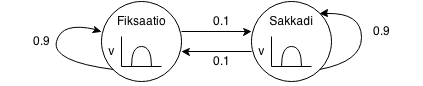
\includegraphics[width=1.0\textwidth]{HMM.png}
		\caption{Markovin piilomalli KORJAA JAKAUMAT!}
		\label{fig:hmm_sample}
\end{figure}

Malli koostuu havainto sekä siirtymätodennäköisyyksistä. Havaintotodennäköisyydet (v jakaumat kuvassa) edustavat tietyn tilan nopeuksien jakaumaa. Ensimmäinen tila edustaa fiksaatiota ja siitä johtuen sen nopeusjakauma on painottunut matalampiin nopeuksiin. Toinen tila edustaa sakkadeja ja vastaavasti sen nopeusjakauma on painottunut suurempiin nopeuksiin. Siirtymätodennäköisyyksiä esittävät kuvassa~\ref{fig:hmm_sample} esiintyvät nuolet ja ne tarkoittavat sitä todennäköisyyttä, jolla tila joko pysyy samana tai muuttuu sakkadista fiksaatioksi tai päinvastoin.

Malli tarvitsee toimiakseen kahdeksan parametria: molempien tilojen nopeusjakaumien keskiarvon ja varianssin sekä todennäköisyydet tilasiirtymille. Vaikka parametreja onkin enemmän kuin esimerkiksi nopeusraja-arvoalgoritmissa niin tämä ei ole ongelma, koska parametrien arvot ovat optimoitavissa harjoitteludatajoukon avulla menetelmällä nimeltä ``HMM uudelleen arviointi'' (HMM reestimation).\citep[s. 180]{salvucci1999} Suurin haaste tämän algoritmin käytössä onkin parametrien optimoinnin implementointi. Tähän olisikin suositeltavaa käyttää jotakin valmista kirjastoa, jos sellainen vain käytettälle ympäristölle on saatavissa.

Kun mallin parametrit on saatu määriteltyä voidaan mallia käyttää arvioimaan jokaiselle datajoukon pisteelle kuuluuko se fiksaatiohin vai sakkadeihin. Luokittelu tehdään HMM-dekoodaus menetelmällä, jossa etsitään todennäköisin sarja tiloja, joka määritellyn mallin perustella syntyy kun sille syötetään uusi datajoukko. Tämän todennäköisimmän sarjan laskentaan voidaan käyttää Viterbin algoritmia.\citep[s. 178]{salvucci1999}  Peräkkäiset fiksaatioiksi luokitellut pisteet yhdistetään myös toisiinsa samalla tavoin kuin nopeusraja-arvoalgoritmissa tehtiin.\citep[s. 31]{salvucci1999} Mallin parametrien optimoinnin jälkeen mallia voidaankin käyttää myös uusien datajoukkojen analysointiin, kunhan datajoukko on kerätty samassa ympäristössä ja olosuhteissa.

Markovin piilomalliin perustuva algoritmi toimii myöskin lineaarisessa ajassa kuten nopeusraja-arvo algoritmi, jotenka sitä voidaan käyttää myös reaaliaikaisuutta vaativissa ympäristöissä. Algoritmi tunnisti myös fiksaatiot tehokkaammin kuin nopeusraja-arvo algoritmi paljon häiriöitä sisältäneestä datasta \citet[s. 32]{salvucci1999}:n tekemässä tutkimuksessa.

\subsection{Pienimpään viritettyyn puuhun perustuva tunnistusalgoritmi I-MST}
I-MST-algoritmi on I-DT algoritmin ohella yksi tunnistusalgoritmeista, joka perustuu datapisteiden sijaintitiedon hyväksikäyttämiselle. Viritetyllä puulla tarkoitetaan puuta, joka kulkee graafin jokaisen pisteen kautta muodostamatta syklejä. Pienin viritetty puu on kaikista mahdollisista viritetyistä puista, joita graafista voidaan muodostaa se puu, jonka sivujen kustannusten muodostama summa on pienin. Sovellettaessa tunnistusalgoritmiin kustannuksella tarkoitetaan etäisyyttä, joka pistellä on toiseen pisteeseen.

Ensimmäiseksi algoritmissa jaetaan datajoukon pisteet osiin niin, että jokaisen osan pituus ajassa on se, mitä arvellaan pisimmän sakkadin datajoukossa olevan. Komogortsev käytti tutkimuksessaan tähän arvoa 200ms.\citep[s. 3 ]{komogortsev2010}. Tämän jälkeen jokaisesta osasta muodostetaan graafi yhdistämällä jokainen osajoukon piste toisiinsa sivulla ja antamalla sivun kustannukseksi pisteiden välinen etäisyys. Kun graafit on muodostettu etsitään jokaisesta graafista pienin viritetty puu. Pienimmän viritetyn puun löytämiseen voidaan käyttää Primin algoritmia.\citep[s. 75]{salvucci2000} Kun pienin viritetty puu on löydetty käydään sen pisteet läpi järjestyksessä jakaen pisteet sakkadeihin tai fiksaatiohin riippuen siitä onko etäisyys edelliseen pisteeseen suurempi vai pienempi kuin asetettu etäisyysraja-arvo.

On huomattava, että kun pienin viritetty puu muodostetaan ja fiksaatioita luokitellaan sen jälkeen, niin tietoa siitä missä järjestyksessä pisteet ovat alkuperäisessä datajoukossa ei oteta huomioon. Koska alkuperäinen datajoukko on alunperin jaettu pieniin osiin ennen puiden muodostamista, niin sillä että tieto puun pisteiden ajallisista suhteista hylätään ei ole juurikaan merkitystä. Itse asiassa tämä hylkääminen on algoritmille hyvä asia, koska silloin se kestää häiriöpisteitä hyvin. Esimerkiksi tilanteessa, jossa meillä on neljä peräkkäistä datapistettä, joista pisteet yksi, kaksi ja neljä ovat lähellä toisiaan ja kolmas piste on häiriöpiste kaukana muista, niin pisteet yksi, kaksi ja neljä tullaan luokittelemaan fiksaatioiksi, koska pisteistä muodostetussa pienimmässä viritetyssä puussa kolmas piste ei tule olemaan muiden pisteiden välissä vaan reunalla, jolloin ei muodostu kuin yksi sakkadiksi luokiteltava piste kahden sijasta, joka tapahtuisi jos käytettäisiin I-VT-algoritmia.

I-MST tarvitsee toimiakseen kaksi parametria: ajan jonka mukaan datajoukko jaetaan pienempiin osiin sekä etäisyysraja-arvon. Komogortsev ei tutkimuksessaan perustellut, mistä hänen käyttämänsä arvo 200ms datajoukon jakamiseen oli saatu muuten kuin, että se oli arvaus pisimmästä sakkadista, joka aineistossa esiintyisi. Parametrin asettamiseen ei siis ole automaattista tapaa vaan tutkija joutuu käyttämään jonkinlaista arvausta lähtökohtana. Etäisyysraja-arvon asettamiseen voitaneen käyttää samaa menetelmää kuin I-VT-algoritmissa vaikkakaan Komogortsev tai Salvucci eivät kumpikaan parametrin asettamista avaa tutkimuksissaan.

I-MST ei nopeudeltaan kilpaile muiden tässä työssä esiteltyjen algoritmien kanssa. Pienimmän viritetyn puun laskemisen kustannus kasvaa ekspotentiaalisesti, mitä enemmän pisteitä puuhun kuuluu. Eli toisin sanoen mitä suurempi näytteenottotaajuus datajoukossa on sitä raskaampaa I-MST-algoritmin käyttäminen on. 

Algoritmin implementointi on selvästi monimutkaisempaa kuin I-VT ja I-DT algoritmien, mutta yksinkertaisempaa kuin I-HMM-algoritmin. Mikäli algoritmia suunnittelee käyttävänsä on suositeltavaa käyttää jotakin kirjastoa, joka osaa laskea pienimmän viritetyn puun annetusta graafista. Tälläisia kirjastoja löytyy varmasti lähes jokaiselle ympäristölle, koska kyseessä on niin perustavanlaatuinen graafialgoritmi.


		\begin{table}
    \begin{tabular}{| p{4cm} | p{3cm} | p{3cm}| p{3.5cm} |}
    \hline
    Algoritmi & Parametrit & Implementoinnin haastavuus & Harjoitustarve \\ \hline
    I-VT nopeusraja-arvo algoritmi & 1 & Erittäin helppo & Ei\\ \hline
    I-DT dispersioraja-arvo algorimiti & 2 & Helppo & Ei \\ \hline
    I-HMM Markovin piilomallia käyttävä algoritmi & 8 / 0 & Haastava & Kyllä \\ \hline
		I-ST Pienimmän viritetyn puun algoritmi & 2 & Kohtuullinen & Ei \\
    \hline
    \end{tabular}
		
		\vspace*{0.2 cm}
		
    \begin{tabular}{| p{4cm} | p{3cm} | p{3cm} |  p{3.5cm} |}
    \hline
    Algoritmi & Nopeus & Häiriönsietokyky & Tunnistus perustuu  \\ \hline
    I-VT nopeusraja-arvo algoritmi  & Erittäin hyvä & Huono  & Nopeus \\ \hline
    I-DT dispersioraja-arvo algorimiti  & Hyvä & Hyvä & Dispersio\\ \hline
    I-HMM Markovin piilomallia käyttävä algoritmi & Hyvä & Hyvä & Nopeus \\ \hline
		I-ST Pienimmän viritetyn puun algoritmi & Kohtuullinen & Hyvä & Dispersio \\
    \hline
    \end{tabular}
		
		\caption{Tunnistusalgoritmien ominaisuuksia}
		\end{table}

\subsection{Metriikoita algoritmien vertailuun}
Jotta erilaisia fiksaationtunnistusalgoritmeja olisi mahdollista verrata toisiinsa, on otettava käyttöön metriikoita, joilla tätä vertailua voidaan tehdä. Seuraavaksi esittelemme kirjallisuudesta löytyneitä menetelmiä vertailujen tekemiseen.

\citet[s. 4]{komogortsev2010} esittelee julkaisussaan erilaisia metriikoita fiksaationtunnistusalgoritmien vertailemiseen. Yksi näistä metriikoista on kvantitatiivinen fiksaatiopisteytys (engl. Fixation Quantitative Score, FQnS). Metriikan käyttämiseen tarvitaan referenssijoukko datapisteitä, joista tiedetään esittävätkö pisteet fiksaatiota vai sakkadeja. Tälläinen datajoukko pitää käytännössä annotoida käsin tai vaihtoehtoisesti voidaan käyttää referenssinä katseentunnituslaitteen annotoimaa dataa niin kuin tässä työssä tullaan tekemään. Metriikan ideana on verrata algoritmin tunnistamien fiksaatioiden määrää referenssijoukossa olevien fiksaatioiden määrään.

\[
FQnS = 100 * {{tunnistettujen\ fiksaatioiden\ lkm} \over {referenssifiksaatiot}}
\]
 
 Metriikan laskennassa käydään jokainen laskettavan datajoukon piste läpi ja mikäli piste on on arvioitu fiksaatioksi niin verrataan sitä vastaavan ajankohdan pisteeseen referenssijoukossa. Mikäli referenssijoukossa tuona ajankohtana oleva piste on fiksaatio niin kasvatetaan tunnistettujen fiksaatioiden määrää yhdellä. On huomattava, että FQnS:n laskennassa ei rangaista, mikäli referenssijoukon sakkadia luullaan fiksaatioksi. Näin ollen pelkästään tätä mittaria maksimoimalla ei saada hyvin toimivaa algoritmia, koska mittari voidaan maksimoida vain arvaamalla kaikki pisteet fiksaatioiksi.
 
 Toinen Komogortsevin julkaisussa esitetty metriikka on nimeltään kvalitatiivinen fiksaatioiden pisteytys (engl. Fixation Qualitative Score, FQlS). Metriikkassa verrataan tunnistettuja fiksaatiopisteitä referenssidataan ja lasketaan keskimääräinen etäisyys, joka oikein tunnistetulla fiksaatiolla ja referenssifiksaatiolla on toisistaan. 

\[
FQlS = {1 \over N} * \sum\limits_{i=1}^N etaisyys\ referenssifiksaatiosta_i
\]

N kuvaa kaavassa oikein tunnistettujen fiksaatiopisteiden määrää. Mitä lähempänä FQlS on nollaa sen parempi, koska tällöin keskimääräinen virhe tunnistetulla fiksaatiolla ja referenssillä on pienin. FQlS ei myöskään rankaise väärin tunnistetuista fiksaatioista, joten myöskään pelkästään FQlS:ää ei kannata käyttää algoritmien tarkkuuksien vertailussa.

Muita enemmän kvantitatiivisia metriikoita, joilla eri algoritmien tuloksia voi verrata toisiinsa ovat esimerkiksi:
\begin{itemize}
  \item keskimääräinen fiksaatioiden määrä (engl. Average Number of Fixations, ANF) \citep[s. 4]{komogortsev2010}
  \item keskimääräinen fiksaatioiden kesto (engl. Average Fixation Duration, AFD) \citep[s. 4]{komogortsev2010}
  \item keskimääräinen sakkadien määrä (engl. Average Number of Saccades, ANS) \citep[s. 4]{komogortsev2010}
	\item keskimääräinen sakkadin voimakkuus (engl. Average Saccade Amplitude, ASA) \citep[s. 4]{komogortsev2010}
	\item sakkadien huippunopeus (engl. Saccade peak velocity) \citep[s. 195]{nystrom2010}
	\item sakkadien huippukiihtyvyys (engl. Saccade peak acceleration) \citep[s. 195]{nystrom2010}
	
\end{itemize}

Edellisillä metriikoiden avulla voidaan huomata algoritmeille tyypillisiä piirteitä niin kuin esimerkiksi \citet[s. 195]{nystrom2010} tekevät artikkelissaan. Artikkelissa nopeusraja-arvoon perustuvalla algoritmilla keskimääräinen fiksaation kesto on lyhyempi kuin muilla vertailtavilla algoritmeilla. Tämän he argumentoivat johtuvan siitä, että algoritmissa ei ole minkäälaista häiriösuodatusta, jolloin yksittäinen häiriöpiste fiksaation sisällä riittää jakamaan fiksaation kahtia.

Luvussa ``Fiksaatioiden tunnistaminen liikedatasta'' tullaan erilaisia fiksaationtunnistusalgoritmeja käyttämään silmänliikedatan luokitteluun ja osaa edellä olevista metriikoista myös algoritmien vertailuun. Koska algoritmien luokittelutuloksia tullaan vertaamaan kaupallisen katseentunnistuslaitteen ohjelmiston tuottamiin tuloksiin on oltava myös metriikka, jolla laskea algoritmin tarkkuutta. FQnS ei sellaisenaan sovellu tarkoitukseen, koska haluamme myös, että väärät luokittelut vaikuttavat metriikan arvoon. Algoritmin  tarkkuutta verrattuna referenssitoteutukseen tullaankin mittaamaan yksinkertaisesti oikeaan osuneiden luokitteluiden suhteella kaikkiin luokiteltavien pisteiden määrään.




\section{Fiksaatioiden tunnistaminen liikedatasta}

\label{sec:esimluku}

 --------------------------------------------------------------------

\section{Johtopäätökset}

Loppuluku päättää työn. Luvun nimi on tyypillisesti ``yhteenveto'' tai
``johtopäätöksiä''. Valitse se otsikko, joka tuntuu sopivammalta työsi
luonteeseen. Joka tapauksessa loppuluku sisältää niin työn yhteenvedon
kuin johtopäätöksiä työn tulosten perusteella. Pääajatus on antaa
lukijalle selvä kuva siitä, miten johdannossa asetettuihin
tavoitteisiin työssä vastattiin.

Käsittele loppupuvussa seuraavia asioita (jotakuinkin tässä järjestyksessä):
%
\begin{itemize}
  \item Muistutus työn tavoitteista (sidoksisuus johdantoon)
  \item Päätulokset kootaan yhteen, pohditaan niiden merkitystä
  \item Suositukset konkreettisiksi toimenpiteiksi (``Mitä sitten?'' 
Nyt kun käytössä on tämän työn myötä tullut tieto, 
mitä se nyt tarkoittaa tälle asialle/alalle.)
  \item Tulosten soveltuvuus, käyttöön liittyvät rajoitukset
  \item Jatkotutkimustarve 
(``Tulevaisuudessa olisi mielenkiintoista selvittää...'' tms.)
  \item Työn onnistumisen arviointi 
(Huom! Älä arvioi omaa kirjoitusprosessiasi vaan tekemääsi tutkimusta)
\end{itemize}

% --------------------------------------------------------------------


%\clearpage                     % luku loppuu, loput kelluvat tänne, sivunv.

%\input{luku2}                  % tässä tyylissä ei sivunvaihtoja lukujen
%\input{luku3}                  %   välillä. Toiset ohjaajat haluavat 
%\input{luku4}                  %   sivunvaihdot.

\label{pages:text}
\clearpage                     % luku loppuu, loput kelluvat tänne, sivunvaihto
%\newpage                       % ellei ylempi tehoa, pakota lähdeluettelo 
                               % alkamaan uudelta sivulta

% -------------- Lähdeluettelo / reference list -----------------------
%
% Lähdeluettelo alkaa aina omalta sivultaan; pakota lähteet alkamaan
% joko \clearpage tai \newpage
%
%
% Muista, että saat kirjallisuusluettelon vasta
%  kun olet kääntänyt ja kaulinnut "latex, bibtex, latex, latex"
%  (ellet käytä Makefilea ja "make")

% Viitetyylitiedosto aaltosci_t.bst; muokattu HY:n tktl-tyylistä.
\bibliographystyle{aaltosci_t}
% Katso myös tämän tiedoston yläosan "preamble" ja siellä \bibpunct.

% Muutetaan otsikko "Kirjallisuutta" -> "Lähteet"
\renewcommand{\refname}{Lähteet}  % article-tyyppisen
%\renewcommand{\bibname}{Lähteet}  % jos olisi book, report-tyyppinen

% Lisätään sisällysluetteloon
\addcontentsline{toc}{section}{\refname}  % article
%\addcontentsline{toc}{chapter}{\bibname}  % book, report

% Määritä kaikki bib-tiedostot
\bibliography{lahteet}
%\bibliography{thesis_sources,ietf_sources}

\label{pages:refs}
\clearpage         % erotetaan mahd. liitteet alkamaan uudelta sivulta

% -------------- Liitteet / Appendices --------------------------------
%
% Liitteitä ei yleensä tarvita. Kommentoi tällöin seuraavat
% rivit.

% Tiivistelmässä joskus matemaattisen kaavan tarkempi johtaminen, 
% haastattelurunko, kyselypohja, ylimääräisiä kuvia, lyhyitä 
% ohjelmakoodeja tai datatiedostoja.

\appendix
\section{Esimerkkiliite}
\label{sec:app1}

Jos työhön kuuluu suurikokoisia (yli puoli sivua) kuvia, taulukoita
tai karttoja tms., jotka eivät kokonsa puolesta sovi tekstin joukkoon,
ne laitetaan liitteisiin. Liitteet numeroidaan. Jokaiseen liitteeseen
tulee viitata tekstissä, eikä liitteisiin ole tarkoitus laittaa ``mitä
tahansa'', vaan vain työlle oikeasti tarpeellista
materiaalia. Liitteisiin voidaan sijoittaa esim. malli
kyselylomakkeesta, jolla tutkimushaastattelu toteutettiin,
pohjapiirustuksia, taulukoita, kaavioita, kuvia tms.

\textbf{TIK.kand suositus: Vältä liitteitä.} Jos iso kuva, mieti onko
sen koko pienettävissä (täytyy olla tulkittavissa) normaalin tekstin
yhteyteen. Joskus liitteeksi lisätään matemaattisen kaavan tarkempi
johtaminen, haastattelurunko, kyselypohja, ylimääräisiä kuvia, lyhyitä
ohjelmakoodeja tai datatiedostoja.

Työtä varten mahdollisesti tehtyjä ohjelmakoodeja ei tyypillisesti
lisätä tänne, ellei siihen ole joku erityinen syy. (Kukaan ei ala
kirjoittaa tai tarkistamaan koko koodia paperilta vaan pyytää sitä
sinulta, jos on kiinnostunut.)

%\subsection{Esimerkkiliitteen otsikko 1}
%\label{sec:app1_1}
%
%Kerätty data-aineisto.
%
% -------------------------------------------------------------- %
%
%\newpage
%\section{Toinen esimerkkiliite}
%\label{sec:app2}
%
%Haastattelukysymykset: mitä, missä, milloin, kuka, miten.



\label{pages:appendices}

% ---------------------------------------------------------------------

\end{document}
